% !TEX program = pdflatex
% Overleaf-compatible. Self-contained: only stock packages.
% Figures live in ./figures/bridge\_tunnel/ (see paper/README.md for how to regenerate).
\documentclass[11pt]{article}

\usepackage[margin=1in]{geometry}
\usepackage{graphicx}
\usepackage{booktabs}
\usepackage{makecell}
\usepackage{float}
\usepackage{amsmath}
\usepackage{amssymb}
\usepackage{xcolor}
\usepackage{caption}
\usepackage{subcaption}
\usepackage{enumitem}
\usepackage{tikz}
\usetikzlibrary{arrows.meta, positioning, fit, backgrounds, calc}

\captionsetup{font=small, labelfont=bf}
\newcommand{\code}[1]{\texttt{#1}}

% block-diagram node styles (shared by the two architecture figures)
\tikzset{
  blk/.style  = {draw, rounded corners, align=center, font=\small,
                 minimum height=2.6em, fill=blue!8, inner sep=4pt},
  head/.style = {draw, rounded corners, align=center, font=\small,
                 minimum height=2.4em, fill=orange!14, inner sep=4pt},
  lat/.style  = {draw, rounded corners, align=center, font=\small,
                 minimum height=2.6em, fill=green!10, inner sep=4pt},
  io/.style   = {draw, rounded corners, align=center, font=\small,
                 minimum height=2.6em, fill=gray!10, inner sep=4pt},
  fl/.style   = {-{Stealth[length=2.2mm]}, thick},
}

\title{\textbf{bridge\_tunnel\_nav}\\[2pt]
\large A POMDP navigation environment with a bridge / mine / detour
strategy choice, built as a substrate for mechanistic interpretability}
\author{}
\date{}

\begin{document}
\maketitle
\vspace{-2.2em}

\begin{abstract}\noindent
\textsc{bridge\_tunnel\_nav} is a small partially-observable navigation environment in
which an agent crosses open procedural terrain to reach a narrow goal door. The
direct route is blocked by obstacles the agent can deal with in three distinct
ways: \textbf{bridge} a lake (place wood on water), \textbf{mine} a mountain
(turn rock to grass), or \textbf{walk around} it. Impassable tree forests line
the top and bottom edges so the agent is funnelled through the obstacle-filled
middle, where it must repeatedly choose among the three strategies. The point of
the design is \emph{not} the navigation itself but the \textbf{internal computation
it induces}: under partial observation the agent must infer the shape and type of
the obstacle ahead (a \emph{belief}) and select a crossing strategy (an
\emph{action mode}). We train two agents on the identical task --- a recurrent PPO
baseline and a pure-JAX DreamerV3 world model --- both reaching $100\%$ success,
and use them as a testbed for probing and \textbf{steering} those belief and
strategy representations in activation space. The concrete target is to make an
agent that solves the task reliably but \textbf{never digs tunnels}, by
suppressing the ``mine'' strategy through an activation-space intervention rather
than an action mask.
\end{abstract}

\section{Idea and motivation}

We want a task that is (i) trivial to solve, so competence is not the bottleneck,
yet (ii) forces a small number of \emph{discrete, legible decisions} that depend
on a \emph{partially-observed latent} (the obstacle ahead). Such a task is an
ideal substrate for mechanistic interpretability: there should be a low-dimensional
\emph{belief} subspace (is the obstacle water or rock; how wide is it) and a
\emph{strategy} subspace (bridge vs.\ mine vs.\ detour) in the agent's recurrent
state, and we can test whether those subspaces are (a) linearly decodable and
(b) \emph{causally} steerable. The headline experiment is suppression: keep the
agent fully competent while removing one option (tunneling) by editing activations
--- the recurrent analogue of the ``cheese vector'' steering result on maze-solving
policy networks.

\paragraph{Two environments.} We study the belief--strategy relationship in two
complementary settings. We \emph{first} present a deliberately \textbf{controlled}
variant, \code{bridge\_tunnel\_commit}, in which both the belief and the skill are
made \emph{explicit and discrete} --- a clean ground-truth map from a labeled belief
to an enforced, committed skill (\S\ref{sec:commit}). We \emph{then} present the
open \code{bridge\_tunnel} task (the remainder of the paper), where neither is
labeled nor enforced: the belief is a continuous, partially-observed inference and
the strategy is a soft, reversible tendency. The controlled variant is the place
to first establish that a belief$\to$skill map exists and is legible; the open task
is where the harder probing/steering programme of \S\ref{sec:mechinterp} lives.

\section{The \code{bridge\_tunnel\_commit} environment: a controlled
belief--skill testbed}\label{sec:commit}

\paragraph{Why a controlled variant.} In the open task (below) the agent's belief
--- the type and size of the obstacle ahead --- is a continuous, noisy inference,
and its ``strategy'' is a soft tendency it can revise mid-obstacle (poke a lake,
back out, detour). That makes \emph{belief} and \emph{skill} useful descriptions
for us, but neither is a clean ground-truth variable to probe against.
\code{bridge\_tunnel\_commit} pins both down while keeping the terrain, observation
format, reward and agents otherwise identical:

\begin{itemize}[leftmargin=1.4em, itemsep=2pt]
\item \textbf{Labeled belief $=$ map category.} Every map belongs to one of three
labeled categories, drawn uniformly: \textsc{balanced} ($14\%/14\%$ water/rock),
\textsc{lakes} (water-dominated, ${\approx}80/20$), and \textsc{rocky}
(rock-dominated, ${\approx}20/80$). The dominant obstacle is the latent the agent
must infer from its egocentric crop, and we hold the exact category label for every
episode (Fig.~\ref{fig:commit-maps}).
\item \textbf{Enforced skill $=$ irreversible commitment.} The action space grows to
\code{Discrete(8)}: the four moves, \code{BUILD} and \code{MINE}, and two new
actions \code{COMMIT\_BUILD} / \code{COMMIT\_MINE}. \code{BUILD}/\code{MINE} are
\textbf{no-ops until the matching commit}. The commitment slot starts \emph{none};
the first commit action sets it and is \emph{irreversible} --- the other tool is
then permanently locked for the rest of the episode. The agent may move freely, but
to ever cross an obstacle it must first commit to exactly one tool. The current
commitment is exposed in the observation scalars
($\mathbb{R}^{7}=[\textsc{facing}(4),\ \text{step}/\text{max},\
\text{committed\_build},\ \text{committed\_mine}]$).
\end{itemize}

\paragraph{The belief$\to$skill map.} Crossing the \emph{abundant} obstacle of a
category is far cheaper than detouring around all of it, so the optimal commitment
is dictated by the category: \textsc{lakes}$\,\to\,$\code{COMMIT\_BUILD},
\textsc{rocky}$\,\to\,$\code{COMMIT\_MINE}, \textsc{balanced}$\,\to\,$either. A
competent agent therefore realises a clean function from a \emph{discrete belief}
(category) to a \emph{discrete, committed skill}. We read this function off directly
as a $3\times3$ \textbf{commit matrix} (Fig.~\ref{fig:commit-matrix}): rows are the
map category, columns are the skill the agent ended the episode committed to
(\textsf{none}/\textsf{build}/\textsf{mine}), and each entry is the fraction of
held-out episodes of that category --- so every row sums to $1$. The ideal,
belief-reading agent puts its mass on the diagonal (build for lakes, mine for
rocky) with a split on the balanced row.

\paragraph{Maps and reward.} Terrain uses the \emph{same} domain-warped fractal
pipeline as the open task (\S\ref{sec:gen}), only with each category's water/rock
fractions; every map is rejection-sampled to be winnable under its intended
commitment. The reward is unchanged (slack $-0.01$, reach $+3$, no build cost, PBRS
shaping with $\gamma{=}0.997$) with one addition: the cost-to-go potential is
\textbf{commitment-aware}. Three Dijkstra fields (none\,/\,build\,/\,mine) are
precomputed per map and indexed by the \emph{live} commitment --- the
\emph{non}-committed obstacle becomes an impassable wall --- and capped at
$2(H{+}W)$ so the potential stays bounded. Committing to the wrong tool therefore
\emph{raises} the cost-to-go (or strands the agent on a one-sided map), so the
shaping itself, together with the sparse reach bonus, teaches the agent to read the
terrain \emph{before} it commits. The pure-JAX port is again proven bit-for-bit
equivalent to the PyTorch env, now across all $8$ actions.

\begin{figure}[H]
\centering

\includegraphics[width=\linewidth]{figures/bridge\_tunnel_commit/categories.png}
\caption{The three labeled map categories (rows) of \code{bridge\_tunnel\_commit},
five seeds each. White dot $=$ spawn; yellow $=$ the 3-cell goal door. \textsc{lakes}
are water-dominated (the cheap crossings are over water $\to$ commit \emph{build}),
\textsc{rocky} are rock-dominated (commit \emph{mine}), \textsc{balanced} is an even
mix (either tool works). The category is the ground-truth \emph{belief} the agent
must infer under partial observation.}
\label{fig:commit-maps}
\end{figure}

\begin{figure}[H]
\centering
\begin{subfigure}{0.49\linewidth}\centering

\includegraphics[width=\linewidth]{figures/bridge\_tunnel_commit/ppo_commit_matrix.png}
\caption{PPO + GRU}
\end{subfigure}\hfill
\begin{subfigure}{0.49\linewidth}\centering

\includegraphics[width=\linewidth]{figures/bridge\_tunnel_commit/dreamer_commit_matrix.png}
\caption{DreamerV3 (25M)}
\end{subfigure}
\caption{The $3\times3$ \textbf{belief$\to$skill commit matrix} for each agent: rows
$=$ map category (the inferred belief), columns $=$ the skill the agent irreversibly
committed to (none/build/mine), entries $=$ fraction of held-out episodes (each row
sums to $1$). Mass on the diagonal (build$\,\leftarrow\,$lakes,
mine$\,\leftarrow\,$rocky) means the agent reads the terrain and commits correctly.}
\label{fig:commit-matrix}
\end{figure}

\begin{figure}[H]
\centering
\begin{subfigure}{0.49\linewidth}\centering

\includegraphics[width=\linewidth]{figures/bridge\_tunnel_commit/ppo_traj.png}
\caption{PPO + GRU}
\end{subfigure}\hfill
\begin{subfigure}{0.49\linewidth}\centering

\includegraphics[width=\linewidth]{figures/bridge\_tunnel_commit/dreamer_traj.png}
\caption{DreamerV3 (25M)}
\end{subfigure}
\caption{Stochastic rollouts on held-out maps, rows $=$ category, columns $=$ seeds.
path $=$ blue, \textcolor{red}{bridge $=$ red}, \textcolor{orange}{mine $=$ yellow},
\textcolor{magenta}{commit step $=$ $\star$}. Each panel is titled with its success
rate and the episode-level commit split.}
\label{fig:commit-traj}
\end{figure}

\paragraph{From controlled to open.} The remainder of the paper studies the original
\code{bridge\_tunnel} task, which removes \emph{both} scaffolds. The belief is no
longer a single labeled category: obstacle \emph{type and size} vary continuously
\emph{within} a map and must be inferred afresh at each obstacle. And the skill is
no longer enforced: there is no commitment, so the agent may bridge one obstacle,
mine the next, detour a third, and even abandon a half-finished crossing. Belief and
strategy survive only as \emph{emergent, soft} variables in the recurrent state ---
which is the harder, more realistic setting the probing and steering programme of
\S\ref{sec:mechinterp} targets.

\section{Environment}

\paragraph{Tiles.} A $9$-tile symbolic vocabulary (no decorative classes, so the
decoder cannot interpolate phantom tiles):
\begin{center}\small
\begin{tabular}{@{}llll@{}}
\toprule
id & tile & role & behaviour\\
\midrule
0 & \code{GRASS}  & open ground & walkable (cost 1)\\
1 & \code{WATER}  & lake        & cross by \emph{bridging} (place $\to$ wood)\\
2 & \code{ROCK}   & mountain    & cross by \emph{mining} (mine $\to$ grass)\\
3 & \code{WOOD}   & placed bridge & walkable\\
4 & \code{TARGET} & goal door   & walkable; stepping on it wins\\
5 & \code{OOB}    & off-map pad & egocentric padding only\\
6 & \code{TREE}   & forest      & \textbf{impassable} (detour only)\\
7 & \code{SAND}   & water fringe & cosmetic, walkable like grass\\
8 & \code{DIRT}   & rock fringe  & cosmetic, walkable like grass\\
\bottomrule
\end{tabular}
\end{center}

\paragraph{Observation (POMDP).} An egocentric crop centred on the agent:
$\code{minimap}\in\{0,\dots,8\}^{V\times V}$ with $V=21$ (off-map cells padded with
\code{OOB}), plus a scalar vector $\code{scalars}\in\mathbb{R}^{5}=[\textsc{facing}
\text{ one-hot}(4),\ \text{step}/\text{max}]$. The agent never sees the whole map,
so the size/type of an obstacle must be \emph{inferred} as it approaches.

\paragraph{Actions.} \code{Discrete(6)}: up / down / left / right (a move also sets
\textsc{facing}), \code{PLACE} (bridge the water cell in front: $\code{WATER}\to
\code{WOOD}$), and \code{MINE} (mine the rock cell in front: $\code{ROCK}\to
\code{GRASS}$). Trees can never be removed.

\section{Task and procedural maps}

Maps are $32\times64$, generated by a domain-warped fractal heightmap thresholded
into lakes (\code{WATER}) and mountains (\code{ROCK}) with cosmetic \code{SAND}/
\code{DIRT} fringes; the left/right edge columns are kept obstacle-free. The
\textbf{spawn} is the centre of the left edge and the \textbf{goal} is a $3$-cell
central door on the right wall ($\code{goal\_half}=1$). Crucially, impassable
\textbf{tree forests are biased heavily toward the top and bottom rows} (about a
$7\!:\!1$ edge-to-middle ratio), which walls off the trivial ``hug the wall to the
door'' route and forces traversal through the obstacle-filled centre.
Figure~\ref{fig:maps} shows the curated validation set.

\begin{figure}[H]
\centering

\includegraphics[width=0.86\linewidth]{figures/bridge\_tunnel/maps.png}
\caption{The 16 validation maps. White dot = spawn (centre-left); yellow = the
3-cell goal door (centre-right). Blue lakes (bridge), grey mountains (mine), dark
forests clustered along the top/bottom edges (detour). The demo plays these exact
maps.}
\label{fig:maps}
\end{figure}

\subsection{Generation algorithm}\label{sec:gen}
Each map is produced deterministically from a single integer seed
(\code{generate\_bridge\_tunnel\_map(orientation="natural", seed)}); the steps are:
\begin{enumerate}[leftmargin=1.4em, itemsep=2pt]
\item \textbf{Domain-warped fractal heightmap.} A multi-octave OpenSimplex field
$h_0$ (base frequency $\max(6,\max(H,W)/4.5)$, five octaves with weights
$1,\tfrac12,\tfrac14,\tfrac18,\tfrac1{16}$) is \emph{domain-warped} by two further
simplex fields (warp amplitude $0.10\max(H,W)$): $h(r,c)=h_0(r+a\,w_r,\,c+a\,w_c)$.
The warp removes grid-aligned, blobby structure and yields organic coastlines.
\item \textbf{Overlaid landforms.} $2$--$4$ lakes (subtract a height bump) and
$2$--$4$ mountains (add one) are stamped, each a soft logistic \emph{disk} or a
multi-lobe \emph{massif}; radii are drawn with a squared (small-biased)
distribution so most features are small with a rare large one. A thin wiggly
\emph{ridge} (capsule field) is added with probability $\tfrac12$.
\item \textbf{Quantile thresholding.} The lowest \code{water\_frac}$=0.14$ fraction
of $h$ becomes \code{WATER}, the highest \code{rock\_frac}$=0.14$ becomes
\code{ROCK}, the rest \code{GRASS}. Thresholding by quantile makes obstacle
coverage exact regardless of the noise realisation.
\item \textbf{Cosmetic fringes.} A sparse one-cell \code{SAND} speckle is dilated
around water and \code{DIRT} around rock (each kept with prob.\ $0.30$/$0.25$);
both behave exactly like grass but visually mark shorelines/scree.
\item \textbf{Edge bands \& endpoints.} The left/right $10$ columns are forced to
\code{GRASS} (clean spawn/goal approaches). Spawn $=(H/2,0)$; the goal is the
$3$-cell door $\{H/2{-}1,H/2,H/2{+}1\}$ on the right wall.
\item \textbf{Edge-biased forests.} About \code{tree\_frac}$\cdot HW$ cells of
impassable \code{TREE} are placed as radius-$1$--$2$ patches. Each patch row is
sampled with a heavy edge bias --- distance-from-nearest-wall $d=\tfrac12 u^3$ with
$u\!\sim\!\mathrm{U}(0,1)$, snapped to the top or bottom edge --- so most forest
sits in the outer ${\sim}15\%$ of rows, leaving the vertical middle open. A
breadth-first \textbf{reachability guard} removes any patch that would wall the
goal off from the spawn.
\item \textbf{Caching.} The dataset is generated once and pickled; the pure-JAX
env additionally precomputes a Dijkstra cost-to-go field per map so its PBRS
potential is a table lookup (and is identical to the PyTorch env by construction).
\end{enumerate}

\paragraph{Why this geometry.} An earlier variant used the \emph{whole} right wall
as the goal; with a free top/bottom border the cheapest route is to hug an edge and
sprint right, and both agents collapsed to wall-hugging with no obstacle crossing.
Making the goal a narrow central door \emph{and} foresting the edges restores the
intended behaviour: the agent must go through the middle and repeatedly choose
bridge / mine / detour. The strategy mix is therefore a property of the map
geometry, not of the exploration schedule.

\section{Reward}

A move-minimising shaped reward with no per-strategy bias:
\[
r_t \;=\; \underbrace{-0.01}_{\text{slack}}
\;+\;\underbrace{\text{shaping}_t}_{\phi=-\,\text{ctg}}
\;+\;\underbrace{3.0\cdot\mathbb{1}[\text{reach door}]}_{\text{terminal}},
\qquad
\text{shaping}_t = 0.015\,\big(\text{ctg}_{t-1}-\gamma\,\text{ctg}_t\big),
\]
with $\gamma=0.997$. The potential $\phi=-\text{ctg}$ uses a \textbf{min-action
cost-to-go}: entering \code{WATER}/\code{ROCK} costs $2$ (build + move), walkable
tiles cost $1$, and \code{TREE} is impassable; \code{ctg} is computed once at reset
by Dijkstra seeded from the goal cell. With per-build cost $0$, crossing and
detouring are valued purely by total action count, so which strategy the agent
picks at a given obstacle is driven by geometry (is bridging/mining shorter than
going around?), exactly the decision we want to study.

\section{Agents}

Both agents train on the \emph{same} task to a shared metric schema. The PyTorch
PPO env (\code{BridgeTunnelEnv}) and the pure-JAX env (\code{BridgeTunnelJaxEnv}) are
proven bit-for-bit equivalent (a parity test asserts identical obs / reward /
termination over thousands of steps), so the DreamerV3 world model trains on
exactly the task the PPO agent does.

\subsection{Recurrent PPO baseline}
A tile-embedding CNN $\to$ GRU recurrent policy (Fig.~\ref{fig:ppo}). The
$V{\times}V$ tile crop ($9$ classes) is embedded ($16$-d) and augmented with two
CoordConv channels, passed through three $3{\times}3$ ReLU convolutions, flattened,
concatenated with the $5$ scalars, and projected to a $256$-d embedding. A
$128$-unit GRU carries memory across the episode; \textbf{this $h_t\in\mathbb{R}^{128}$
is the POMDP belief carrier and the primary probing target}. Two linear heads read
it: a categorical actor over the $6$ actions and a scalar value. There is \emph{no}
auxiliary belief head --- bridge/mine/detour is driven purely by reward. Entropy
$0.045$, no annealing (keeps the stochastic policy spread out). Adam
($\text{lr}=3\!\times\!10^{-4}$), GAE ($\gamma{=}0.997,\lambda{=}0.95$), clip $0.2$.

\begin{figure}[H]
\centering
\resizebox{\linewidth}{!}{%
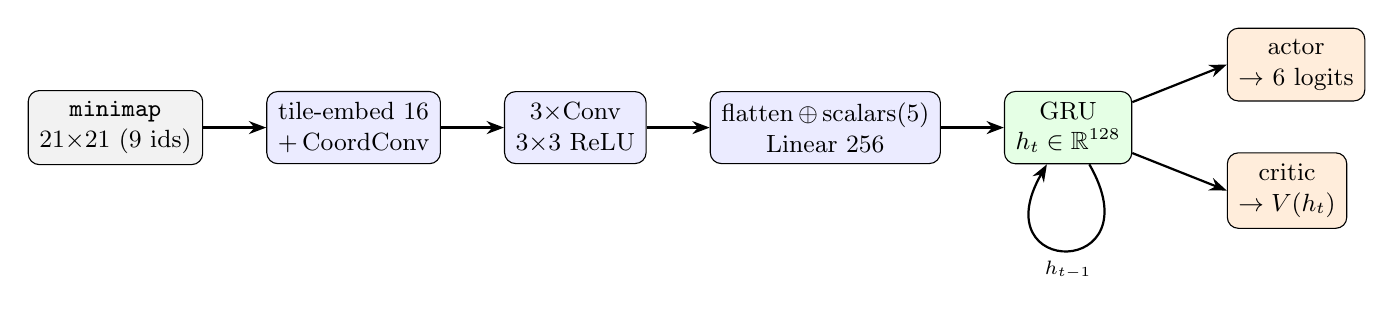
\begin{tikzpicture}[node distance=6mm and 8mm]
  \node[io]  (obs)  {\texttt{minimap}\\$21{\times}21$ (9 ids)};
  \node[blk, right=of obs] (emb) {tile-embed $16$\\$+$\,CoordConv};
  \node[blk, right=of emb] (cnn) {$3\times$Conv\\$3{\times}3$ ReLU};
  \node[blk, right=of cnn] (fc)  {flatten\,$\oplus$\,scalars$(5)$\\Linear $256$};
  \node[lat, right=of fc]  (gru) {GRU\\$h_t\in\mathbb{R}^{128}$};
  \node[head, right=12mm of gru, yshift=8mm]  (act) {actor\\$\to$ 6 logits};
  \node[head, right=12mm of gru, yshift=-8mm] (val) {critic\\$\to V(h_t)$};
  \draw[fl] (obs)--(emb); \draw[fl] (emb)--(cnn); \draw[fl] (cnn)--(fc);
  \draw[fl] (fc)--(gru);
  \draw[fl] (gru)--(act.west); \draw[fl] (gru)--(val.west);
  \draw[fl] (gru) to[out=-60,in=-120,looseness=8]
            node[below,font=\scriptsize]{$h_{t-1}$} (gru);
\end{tikzpicture}}
\caption{PPO+GRU policy. The $5$ scalars are the \textsc{facing} one-hot$(4)$ plus
the step fraction. The $6$ actions are up/down/left/right/\textsf{place}/\textsf{mine}.
The recurrent $h_t$ is the only place the partially-observed obstacle ahead can be
integrated, hence the probing target.}
\label{fig:ppo}
\end{figure}

\subsection{DreamerV3 world model (25M)}
The in-tree pure-JAX \code{purejaxwm} library learns a recurrent state-space model
(RSSM) and trains the actor--critic purely \emph{in imagination}
(Fig.~\ref{fig:dreamer}). Because the minimap is symbolic, the encoder/decoder are
$4$-block MLPs (RMSNorm\,$+$\,SiLU) over the flat $V{\cdot}V+5$ observation vector
--- no pixel CNN. Heads read the RSSM features $[h_t,z_t]$: a decoder
$\hat o_t$, TwoHot reward/continue heads, and the actor/critic optimised on imagined
$\lambda$-returns with a slow (EMA) critic.

\begin{figure}[H]
\centering
\resizebox{\linewidth}{!}{%
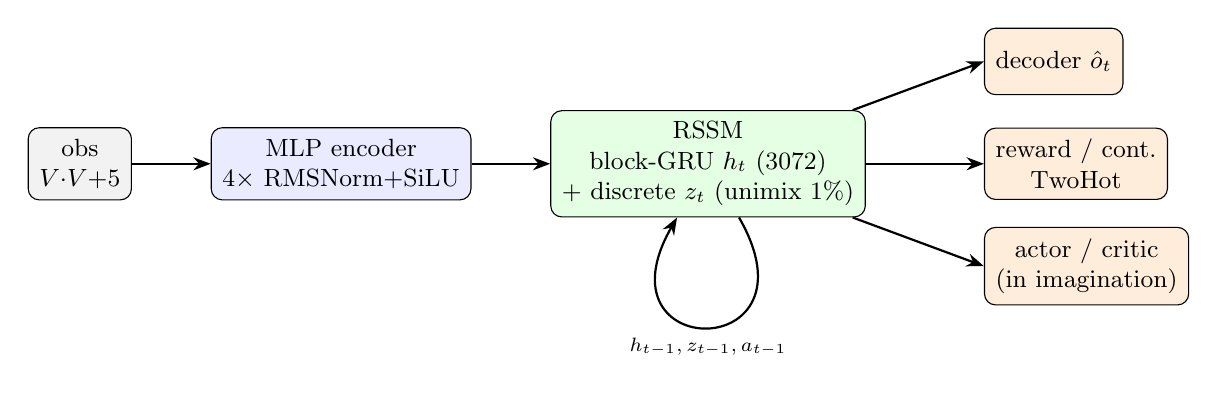
\begin{tikzpicture}[node distance=6mm and 10mm]
  \node[io]  (obs)  {obs\\$V{\cdot}V{+}5$};
  \node[blk, right=of obs] (enc) {MLP encoder\\$4\times$ RMSNorm+SiLU};
  \node[lat, right=of enc] (rssm) {RSSM\\block-GRU $h_t$ ($3072$)\\$+$ discrete $z_t$ (unimix $1\%$)};
  \node[head, right=15mm of rssm, yshift=13mm] (dec) {decoder $\hat o_t$};
  \node[head, right=15mm of rssm, yshift=0mm]  (rew) {reward / cont.\\TwoHot};
  \node[head, right=15mm of rssm, yshift=-13mm](ac)  {actor / critic\\(in imagination)};
  \draw[fl] (obs)--(enc); \draw[fl] (enc)--(rssm);
  \draw[fl] (rssm)--(dec.west); \draw[fl] (rssm)--(rew.west); \draw[fl] (rssm)--(ac.west);
  \draw[fl] (rssm) to[out=-60,in=-120,looseness=7]
            node[below,font=\scriptsize]{$h_{t-1},z_{t-1},a_{t-1}$} (rssm);
\end{tikzpicture}}
\caption{High-level DreamerV3. The RSSM rolls forward in latent space; the
actor--critic is trained on imagined trajectories ($\gamma{=}0.997,\lambda{=}0.95$,
TwoHot over $255$ symlog bins, RetNorm scaling, LaProp $+$ AGC, $\text{lr}=4\mathrm{e}{-5}$).
The $h_t$ ($3072$-d for the 25M preset) $+$ discrete $z_t$ are the latent we probe.}
\label{fig:dreamer}
\end{figure}

\subsection{A fair comparison}\label{sec:fair}
To compare the two algorithms cleanly we train them on the \emph{identical}
environment \emph{and} the \emph{identical observation}: both consume a
\textbf{categorical one-hot} minimap ($V{\times}V{\times}9$). For PPO this replaces
the learned tile embedding with one-hot channels into the CoordConv CNN; for
DreamerV3 it replaces the ordinal-scalar encoder/decoder with a one-hot encoder
and a per-cell cross-entropy decoder (\S\ref{sec:imagination}). Only the
\emph{algorithm} then differs. Table~\ref{tab:agents} reports held-out
trajectory-grid success ($200$ stochastic rollouts $\times$ 6 maps);
Figure~\ref{fig:curves} shows the training curves.

\begin{table}[H]
\centering\small
\begin{tabular}{@{}lcccc@{}}
\toprule
agent & observation & success (held-out) & return & episode length\\
\midrule
PPO + GRU       & one-hot & $100\%$ & ${\approx}3.4$ & ${\approx}89$\\
DreamerV3 (25M) & one-hot & $85\%$  & ${\approx}2.1$ & longer / variable\\
\bottomrule
\end{tabular}
\caption{Both on the same env + same categorical observation (only the algorithm
differs). DreamerV3 logs ${\approx}96\%$ success \emph{during} training but
${\approx}85\%$ in clean per-episode evaluation at $1$M steps (it was only
${\approx}7\%$ at $500$k --- door-homing on the narrow $3$-cell goal is what the
extra budget buys).}
\label{tab:agents}
\end{table}

\begin{figure}[H]
\centering

\includegraphics[width=\linewidth]{figures/bridge\_tunnel/training_curves.png}
\caption{Reward and success vs.\ environment steps (W\&B, rolling). On this
symbolic task \textbf{PPO+GRU is markedly more sample-efficient} --- ${\sim}100\%$
by ${\sim}0.2$M steps --- while DreamerV3 rises more slowly (with a mid-training
dip near $0.5$M) to ${\sim}96\%$ by $1$M. PPO trained to $2$M, DreamerV3 to $1$M.}
\label{fig:curves}
\end{figure}

\section{Behaviour: stochastic rollouts}

Figure~\ref{fig:grids} overlays $200$ stochastic rollouts per map for each agent.
The forests pin the paths into a central corridor; within it the agents bridge
(red), mine (yellow), and detour around the larger masses. Figure~\ref{fig:strat}
isolates one clean rollout of each strategy from the PPO agent --- the three
behaviours we want to find and manipulate internally.

\paragraph{What counts as a crossing (strict).} We label a trajectory segment as
\emph{bridging} or \emph{tunnelling} only when the path \textbf{enters an obstacle
body and exits the other side}: a maximal run of consecutive path cells whose
original terrain is \code{WATER} (resp.\ \code{ROCK}), with at least $2$ distinct
cells \emph{and} distinct entry/exit land cells. Placing or mining a single block,
or poking into a lake and backing out the same side, does \emph{not} count --- it
is still ``avoid''. This is deliberately stricter than counting build/mine events,
and it is exactly the segment-labelling rule we will use for the strategy labels in
the activation dataset (\S\ref{sec:mechinterp}).

\begin{figure}[H]
\centering
\begin{subfigure}{0.49\linewidth}\centering

\includegraphics[width=\linewidth]{figures/bridge\_tunnel/ppo_traj.png}
\caption{PPO + GRU}
\end{subfigure}\hfill
\begin{subfigure}{0.49\linewidth}\centering

\includegraphics[width=\linewidth]{figures/bridge\_tunnel/dreamer_traj.png}
\caption{DreamerV3}
\end{subfigure}
\caption{$200$ stochastic rollouts per map. path = dark blue, \textcolor{red}{bridge
= red}, \textcolor{orange}{mine = yellow}. Both agents funnel through the
forest-walled central corridor and cross obstacles there.}
\label{fig:grids}
\end{figure}

\begin{figure}[H]
\centering

\includegraphics[width=0.95\linewidth]{figures/bridge\_tunnel/strategy_examples.png}
\caption{One stochastic rollout per strategy (PPO agent), under the strict
crossing definition. The crossed lake/mountain body is shaded; the bold segment is
the in$\to$out traversal (green \textbullet\ = entered the body, magenta $\star$ =
exited the far side), the thin blue line is the rest of the path. \textbf{Avoid}
traverses no obstacle body; \textbf{Bridge} crosses a multi-cell lake ($18$ water
cells here); \textbf{Tunnel} crosses a mountain ($16$ rock cells). Over sampled
reaching rollouts the mix is roughly avoid:bridge:tunnel $\approx 1\!:\!2\!:\!0.8$,
so all three modes are well represented.}
\label{fig:strat}
\end{figure}

\section{DreamerV3 imagination}\label{sec:imagination}

Because DreamerV3 learns a world model, we can roll it forward \emph{in
imagination}: condition the RSSM on a few real frames, then let it predict the
rest open-loop (prior only, no further observations) while the chosen actions
still drive the real env, and decode each latent back to an egocentric view. The
minimap is decoded with a \textbf{per-cell categorical (cross-entropy) head} over
the $9$ tiles (the categorical observation of \S\ref{sec:fair}).
Figure~\ref{fig:dream} compares the model's decode (top) against the
\textbf{ground-truth} env observation (bottom) on a demo map.

\begin{figure}[H]
\centering

\includegraphics[width=\linewidth]{figures/bridge\_tunnel/dreamer_imagine_strip.png}
\caption{Open-loop prediction vs.\ reality on a demo map (sprites). \textbf{Top
row} = the model's decoded egocentric view; \textbf{bottom row} = the
ground-truth env observation at the same step. \textcolor{green!60!black}{Green}
columns are the closed-loop warmup (posterior conditioned on the real obs, so the
top row is a faithful \emph{reconstruction}); \textcolor{red}{red} columns are
open-loop imagination (prior only). The reconstruction tracks reality closely;
the open-loop prediction stays plausible (grass/water/rock) but drifts from the
true map --- it does not reproduce the tree cluster and occasionally hallucinates
off-map (black) cells. (Note: the top warmup frames are decoder reconstructions,
\emph{not} the raw observation --- which is exactly the bottom row.)}
\label{fig:dream}
\end{figure}

\paragraph{Why categorical (relevant to probing).} An earlier version encoded the
minimap as a single \emph{ordinal scalar} per cell ($\text{tile\_id}/\text{NUM\_TILES}$)
and \emph{regressed} it with MSE. That produced blurry reconstructions and
\emph{phantom out-of-vocab tiles}: a value between, say, rock$(2)$ and wood$(3)$
rounds to an id that never occurs. The categorical one-hot encoder $+$ per-cell
cross-entropy decoder removes both pathologies --- reconstructions are crisp and
can only emit real tiles (above) --- at a modest cost in policy sample-efficiency
(Fig.~\ref{fig:curves}). The residual divergence in the open-loop frames is
therefore \emph{dynamics} error (the RSSM prediction), not a decoding artifact.
For the interpretability work this matters: the decode is now a genuine per-cell
tile belief, but we will still probe the latent ($h,z$) directly rather than read
beliefs off the decoder.

\section{Mechanistic-interpretability plan}\label{sec:mechinterp}

The agents above are the substrate. The intended programme:
\begin{enumerate}[leftmargin=1.4em]
\item \textbf{Activation dataset.} Fix one or two maps, sample many stochastic
trajectories (logging seed + full metadata), and record the GRU state $h_t$ (and
the pre-recurrent encoder embedding) at every step, labelled with the
ground-truth belief (obstacle type/size ahead) and the committed strategy
(avoid / bridge / tunnel) at each obstacle.
\item \textbf{Probe.} Fit linear probes / difference-of-means directions for the
belief and strategy variables; report decoding accuracy by site, and validate with
unsupervised structure (PCA / clustering).
\item \textbf{Steer.} Add / clamp those directions during fresh rollouts and
measure the causal behavioural change (a probe that decodes but does not steer is
suspect).
\item \textbf{Suppress.} Derive the ``mine'' direction from the \emph{decision}
contrast (mined vs.\ went-around on the same rock obstacle), apply it conditionally,
and verify the agent re-routes via its own bridge/detour policy rather than
failing --- i.e.\ a competent agent that \textbf{never digs tunnels}, achieved in
activation space.
\end{enumerate}

\paragraph{Reproduce.} Train: \code{scripts/train\_ppo\_bridge\_tunnel.py --config
models/bridge\_tunnel\_nav/natural\_centergoal3.yaml} and \code{scripts/dreamerv3\_bridge\_tunnel\_nav.py
--size 25M}. Visualise: \code{scripts/bridge\_tunnel\_traj\_grid.py},
\code{scripts/bridge\_tunnel\_strategy\_examples.py}, \code{scripts/viz\_dreamer\_bridge\_tunnel\_imagine.py}.
See \code{docs/bridge\_tunnel\_nav.md} and \code{docs/codebase\_map.md}.

\end{document}
